\documentclass[runningheads]{llncs}

\usepackage[T1]{fontenc}
\usepackage{newtxtext}
\usepackage[varvw]{newtxmath}
\usepackage{cite}
\usepackage{amsmath,amssymb,amsfonts}
\usepackage{graphicx}
\usepackage{textcomp}
\usepackage{xcolor}
\usepackage{booktabs}
\usepackage{array}
\usepackage{multirow}
\usepackage{makecell}
\usepackage{tabularx}
\usepackage{adjustbox}
\usepackage{algorithm}
\usepackage{algpseudocode}
\usepackage{float}
\usepackage[hidelinks]{hyperref}
\floatplacement{algorithm}{htbp}

\begin{document}

\title{Multilingual and Cross Lingual Speech Emotion Recognition with Wav2Vec2: An English Hindi Study}

\titlerunning{Multilingual and Cross Lingual English Hindi SER Using Wav2Vec2}

\author{Sudipta Bhattacharya\inst{1} \and
Sandipan Sahu\inst{2} \and
Anik Chiney\inst{1} \and
Farhan Wajid\inst{1} \and
Aritra Adhikary\inst{1} \and
Samarjeet Borah\inst{3}\thanks{Corresponding author. Email: samarjeet.b@smit.smu.edu.in}}

\authorrunning{S. Bhattacharya et al.}

\institute{IEM Centre of Excellence for Cloud Computing and IoT, Department of CSE (AIML), Institute of Engineering \& Management, Saltlake, School of University of Engineering and Management, Kolkata-700091, India.\\
\email{\{bhattacharya.sudipta, anikchiney130, farhanwajid05, aritrakemail\}@gmail.com}
\and
Department of CSE, ASETK,
Amity University Kolkata, India\\
\email{sahusandipan@gmail.com}
\and
Department of Computer Applications,
Sikkim Manipal Institute of Technology, Sikkim Manipal University,
Majitar 737136, Sikkim, India\\
\email{samarjeet.b@smit.smu.edu.in}}

\maketitle

\begin{abstract}
Speech Emotion Recognition is a crucial component of Human Computer Interaction and its practical applications, enabling computers to interpret affective information from voice signals and interact more naturally with users. However, most existing studies are restricted to a single language, so the performance of automatic SER systems degrades considerably in multilingual and cross lingual scenarios, particularly for previously unseen, low resource languages such as Hindi. This paper investigates multilingual and cross lingual SER using English (RAVDESS) and Hindi (IESC) datasets with the Wav2Vec 2.0 self supervised model.

Direct (zero shot) cross lingual transfer between the two languages is found to perform poorly, whereas fine tuning on the target language yields a substantial improvement in recognition accuracy. Multilingual training, in which  model is jointly trained on both languages, is further observed to outperform the cross lingual configurations on both datasets.

Overall, this study examines English-Hindi SER, identifies the challenges arising from the language gap, and discusses possible directions for improving performance in low resource settings.

\keywords{Speech Emotion Recognition \and Cross Lingual Transfer \and Multilingual Learning \and Wav2Vec 2.0 \and RAVDESS \and IESC \and Fine Tuning \and Low Resource Languages}
\end{abstract}


\section{Introduction}

Emotion is fundamental aspect of communication and manifests in speech through cues like pitch, energy, rhythm, pauses. Speech Emotion Recognition (SER) aims to detect these emotions automatically from audio signals, enabling computers interact with users in more natural, human way \cite{b1,b2}.

Machine learning (ML) and transformer based learning models play an important role in speech and audio based intelligent systems designed for effective human-computer interaction (HCL) \cite{b16,b17}. SER has attracted considerable research interest in recent years owing its potential applications in robotics, business, education, virtual assistants, customer mood analysis in call centres, mental health monitoring, and stress detection \cite{b17}. Earlier research addressed emotional state identification using classical machine learning models such as K-Nearest Neighbour (KNN), Artificial Neural Networks (ANN), Hidden Markov Models (HMM), Gaussian Mixture Models (GMM), and Support Vector Machines (SVM), together with a variety of handcrafted speech features \cite{b9,b15}. Such systems perform reasonably well when trained and tested on the same corpus, but their performance degrades considerably when tested on speech from different corpus or language \cite{b7,b9}. Cross-corpus SER is particularly challenging because of differences in corpus language, speaker age, labelling schemes, recording conditions, all of which can substantially affect model performance across databases \cite{b7,b9}. This motivates the development of more robust emotion recognition systems capable of handling corpus data spanning multiple languages \cite{b4,b14}, which in turn would facilitate the deployment of SER systems for a wide range of health related and industrial applications \cite{b17}.

Despite these efforts, SER continues to face practical challenges arising from linguistic and cultural differences \cite{b1,b3}. Existing methods remain disadvantaged under noisy conditions, with small datasets, and in fully capturing the intricate patterns present in emotional speech \cite{b23}. Most studies have focused on a single corpus without considering cross corpus or multi corpus effects \cite{b9,b13}, partly because relatively few emotional speech corpora exist compared with number of spoken languages worldwide. In addition, the available resources are highly diverse even within the English language, which contributes to the data sparsity problem widely reported in SER research \cite{b4,b12}. As a result, models often perform poorly in mixed language settings \cite{b7,b8}, making it difficult for an SER system trained on a single data source to operate reliably in real time across languages. Practical deployment therefore requires models that can learn effectively from multiple resources across different languages \cite{b3,b4}.

This paper addresses this gap through experiments on English (RAVDESS) and Hindi (IESC) speech emotion corpora. Cross corpus and multi corpus SER have been studied by several researchers to improve classification accuracy across languages \cite{b7,b9}, using a variety of publicly available datasets to highlight trends in multilingual and cross lingual evaluation \cite{b1,b4}. In this work, Wav2Vec 2.0 transformer model is employed, a state of the art approach for self supervised speech representation learning \cite{b16,b23}. The deep contextual representations learned by Wav2Vec 2.0 directly from raw audio signals eliminate need for hand engineered feature extraction and improve robustness to noise and speech variability \cite{b16,b23}. The primary objective of this research is to develop an improved SER system for the Hindi and English languages. To this end, several experimental scenarios are evaluated using the Wav2Vec 2.0 transformer model \cite{b17}, including zero shot cross lingual transfer (without Hindi training data) and fine tuned transfer, in order to characterise the performance gap between English and Hindi.

Major contributions of this paper are summarised as follows:
\begin{itemize}
\item A systematic evaluation of zero shot cross lingual SER transfer between English (RAVDESS) and Hindi (IESC) using the pretrained Wav2Vec 2.0 model.
\item An analysis of effect of target language fine tuning on cross lingual SER performance for both English and Hindi.
\item A multilingual training framework in which Wav2Vec 2.0 is jointly trained on English and Hindi, and its performance is compared against the cross lingual configurations.
\item A detailed discussion of the linguistic and acoustic factors that contribute to the performance gap between high resource and low resource languages in SER.
\end{itemize}

Remainder of paper is organized as. Section~\ref{sec:related} reviews related work. Section~\ref{sec:methodology} describes the datasets, feature extraction methods, and model architectures. Section~\ref{sec:results} presents experimental results, Section~\ref{sec:discussion} discusses the findings, and Section~\ref{sec:conclusion} concludes paper and outlines future research directions.


\section{Literature Review}
\label{sec:related}

Speech emotion recognition (SER) plays an important role in current human-computer interaction applications, including virtual assistants, emotion sensing technologies, and mental health screening \cite{b17}. Most existing SER systems, however, are trained solely on English datasets and therefore perform poorly on other languages \cite{b3,b4}. Cross lingual SER addresses this limitation by transferring emotion related knowledge from resource rich languages to resource poor ones, thereby reducing the dependence on large labelled datasets \cite{b8,b12}.

Early approaches relied on hand crafted acoustic features together with techniques to reduce discrepancies between datasets \cite{b9,b15}. While partially effective, these methods struggled to isolate genuine emotion related cues from language specific acoustic characteristics \cite{b7,b14}. The subsequent adoption of deep learning architectures, including CNNs and BiLSTM networks, improved pattern learning but still required substantial amounts of target language data \cite{b9,b13}. In this direction, a deep learning based analysis of speech emotion recognition was carried out using convolutional and recurrent architectures to model emotion specific acoustic patterns directly from speech features, showing that deep architectures can capture discriminative emotional cues more effectively than conventional hand crafted feature based classifiers \cite{b18}.

A significant shift occurred with the emergence of self supervised speech models such as Wav2Vec 2.0, HuBERT, WavLM, XLS-R \cite{b16,b27}. These models are pretrained on large-scale multilingual speech corpora, producing acoustic representations that transfer effectively across languages \cite{b16,b27}. Prior studies show that embeddings derived from such models substantially improve zero shot and few shot emotion recognition \cite{b11,b23}.

Recent research directions include multimodal transformers that combine speech and text, phonetic strategies for improved layer wise transfer, domain specific emotion embeddings, and contrastive learning approaches based on large language models \cite{b1,b3}. Parameter efficient fine tuning techniques such as LoRA and adapter modules have also been explored to retain pretrained knowledge while adapting models for SER \cite{b2}. Building further on cross lingual generalization, a cross lingual deep learning framework for gender based emotion detection was proposed, in which gender specific and emotion specific cues were jointly modelled within a single deep learning architecture, and the framework was shown to generalize across languages while improving emotion recognition performance relative to gender agnostic baselines \cite{b22}.

Nevertheless, most existing work remains focused on European languages, while low resource languages such as Hindi receive comparatively little attention \cite{b4,b12}. In particular, zero shot cross lingual transfer of Wav2Vec 2.0 from English to Hindi has not been systematically examined in the literature.

This study addresses this gap by evaluating emotion transfer from English (RAVDESS) to Hindi (IESC) using Wav2Vec 2.0, considering both zero shot transfer and fine tuning between these linguistically distinct languages \cite{b3,b16}. Table~\ref{tab:related_works} shows representative related work in cross lingual and multilingual SER.

\begin{table*}[htbp]
\caption{Summary of related work on cross lingual speech emotion recognition}
\label{tab:related_works}
\centering
\renewcommand{\arraystretch}{1.5}
\setlength{\tabcolsep}{4pt}
\resizebox{\textwidth}{!}{%
\begin{tabular}{|p{2.0cm}|p{3.2cm}|p{2.6cm}|p{4.2cm}|p{4.2cm}|}
\hline
\makecell[l]{\textbf{Author \&}\\\textbf{Year}} &
\makecell[l]{\textbf{Approach /}\\\textbf{Model}} &
\makecell[l]{\textbf{Dataset /}\\\textbf{Languages}} &
\textbf{Key Contribution} &
\textbf{Findings} \\
\hline
Zaidi et al., 2023 \cite{b1} &
Multimodal Dual Attention Transformer &
Multilingual &
Combines audio and text using dual attention &
Multimodal transformers improve emotion recognition accuracy \\
\hline
Latif et al., 2023 \cite{b7} &
Self supervised Adversarial Domain Adaptation &
Cross corpus and cross lingual &
Uses adversarial training for domain invariance &
Achieves robust cross lingual performance across datasets \\
\hline
Bhattacharya et al., 2022 \cite{b18} &
Deep Learning based Analysis (CNN/RNN) &
Single language SER &
Analyzes deep learning architectures for speech emotion recognition using acoustic features &
Deep architectures effectively capture emotion specific acoustic patterns \\
\hline
D'Asaro et al., 2024 \cite{b11} &
SSL Feature Extraction (Wav2Vec2) &
Cross lingual &
Uses pretrained speech models for feature extraction &
SSL features outperform handcrafted features in SER \\
\hline
Babu et al., 2021 \cite{b16} &
XLS-R Transformer &
Multilingual (128 languages) &
Large scale cross lingual speech representation learning &
Strong generalization across multiple languages \\
\hline
Sharma, 2022 \cite{b17} &
Wav2Vec2 Multi task Learning &
Multilingual &
Multi task learning with pretrained transformer &
Improves emotion recognition using shared representations \\
\hline
Bhattacharya et al., 2024 \cite{b22} &
Cross-lingual Deep Learning Model &
Cross lingual, gender based &
Jointly models gender and emotion cues within a deep learning framework &
Gender aware modelling improves cross lingual emotion detection performance \\
\hline
Shendabadi et al., 2026 \cite{b28} &
Whisper + Attentive Pooling &
Multilingual (English, Persian) &
Uses large pretrained speech models for SER &
Large scale models improve multilingual SER performance \\
\hline
\end{tabular}%
}
\end{table*}


\section{Methodology}
\label{sec:methodology}

The RAVDESS and IESC datasets were selected for this study, as their combination offers a suitable mixture of acted emotional expressions recorded under controlled (RAVDESS) and semi controlled (IESC) studio environments. Since classification experiments require training, testing data to share same class labels, four common emotions were selected to maintain consistency between training and testing: Angry, Happy, Sad, and Neutral.  Overall experimental framework is illustrated in Fig.~\ref{fig:framework}.

\subsection{Datasets and Emotion Classes}

\subsubsection{RAVDESS.}
 Ryerson Audio-Visual Database of Emotional Speech and Song (RAVDESS) is widely used multimodal speech emotion corpus. It is recorded in North American English by 24 professional actors (12 male and 12 female) and contains eight emotion labels: Neutral, Calm, Happy, Sad, Angry, Fearful, Disgust, and Surprised, with two intensity levels (normal and strong) for all labels except Neutral. The complete dataset comprises 7,356 recordings spanning speech and song modalities; in this study, only the speech only subset, consisting of 1,440 audio files, is used, and only four emotion categories are utilized.

\subsubsection{IESC.}
Indian Emotional Speech Corpus (IESC) is an Indian emotional speech dataset developed to support SER research for Indian speakers. It is in the Hindi language, with recordings collected from native Indian speakers under controlled conditions. It contains five emotion labels: Neutral, Happy, Sad, Angry, and Fearful, with recordings of 10 speakers (5 male and 5 female) totalling approximately 1,200 audio files. As with RAVDESS, only four emotion categories from this corpus are used in this study.

\begin{figure*}[htbp]
  \centering
  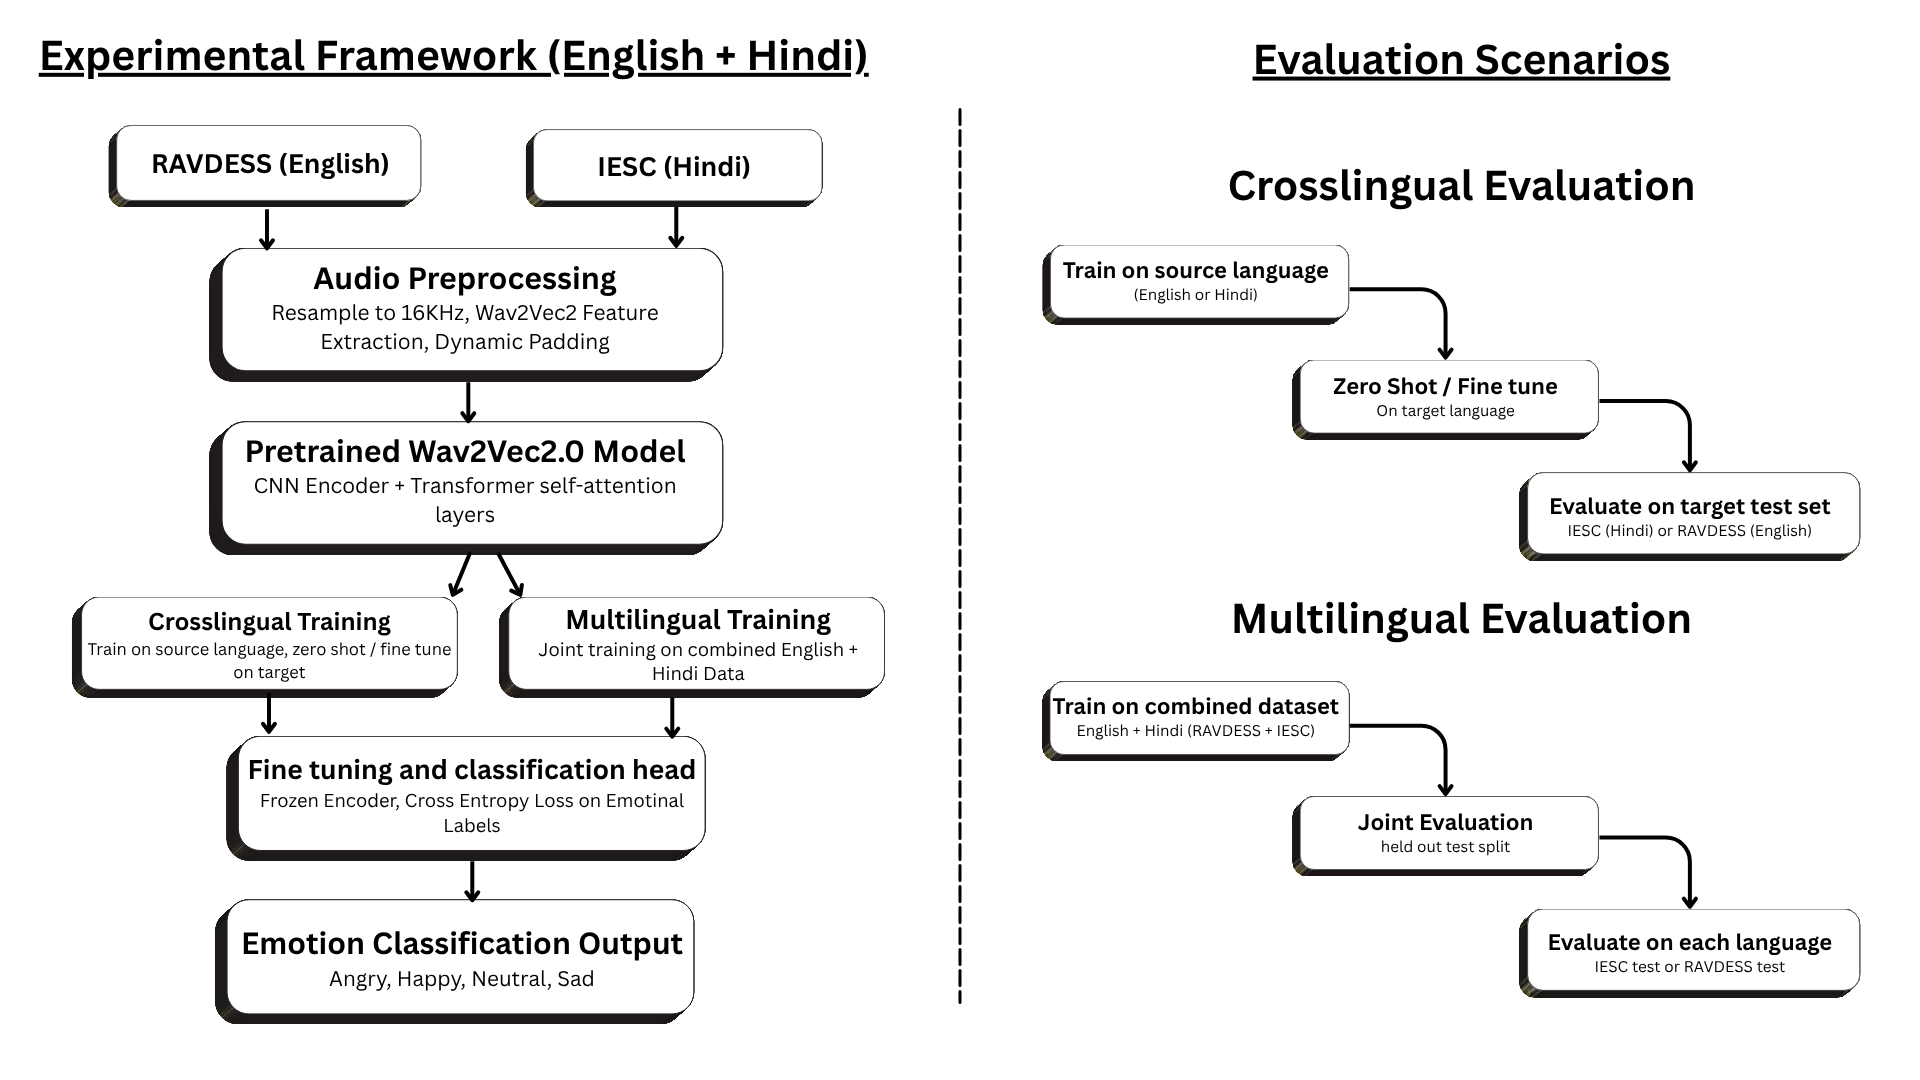
\includegraphics[width=\textwidth]{framework_figure.png}
  \caption{Left: experimental framework for English-Hindi cross lingual and multilingual SER. Right: evaluation scenarios considered, namely cross lingual versus multilingual SER.}
  \label{fig:framework}
\end{figure*}

\subsection{Audio Preprocessing}

For both cross lingual and multilingual analysis, audio preprocessing was performed prior to model training to ensure consistency across the datasets.

The datasets were first loaded from their respective source folders, and each audio file was read in waveform format and resampled to 16 kHz, sampling rate expected by pretrained Wav2Vec2 model. Resampling ensures a uniform temporal resolution across recordings originating from different datasets.

The resampled waveforms were then converted into floating point representations using the pretrained Wav2Vec2 processor (feature extractor), which produces model compatible input representations directly from raw waveforms. Unlike conventional feature extraction methods like MFCCs, Wav2Vec2 operates directly on the input waveform and internally learns hierarchical speech representations through self supervised pretraining.

A data collator was employed to apply dynamic padding during batch formation, allowing utterances of varying lengths to be handled efficiently while reducing unnecessary computational overhead and maintaining compatibility with transformer based architectures.

\subsection{Model Classification}

For cross lingual and multilingual SER, pretrained Wav2Vec2 based sequence classification framework suitable for raw speech waveforms is used. The model consists of CNN-based feature encoder that extracts low level acoustic features such as pitch, energy, and temporal dynamics from the raw waveform. These latent features are subsequently passed through multi layer transformer encoder that captures long range temporal dependencies via self attention. A task specific linear classification layer is added on pooled transformer representations, mapping contextual speech embeddings to predefined emotion categories, with the output layer dimension adjusted according to the number of classes required for each experimental setup. Algorithm~\ref{alg:crosslingual} summarizes the zero shot cross lingual evaluation procedure.

\begin{algorithm}[htbp]
\caption{Cross lingual SER using Wav2Vec2}
\label{alg:crosslingual}
\begin{algorithmic}[1]
\Require English dataset $D^E$, Hindi dataset $D^H$, pretrained Wav2Vec2 model $f(\cdot)$
\Ensure Cross lingual accuracy $Acc^H$
\State Preprocess audio signals $x \in D^E \cup D^H$ (resample to 16\,kHz)
\State Convert waveform to input features using Wav2Vec2 processor
\State Load pretrained Wav2Vec2 model $f(\cdot)$
\State Fine tune model on English dataset $D^E$
\State Freeze feature encoder and update classification layers
\State Evaluate model directly on Hindi dataset $D^H$ (zero shot)
\State Compute cross lingual accuracy $Acc^H$
\end{algorithmic}
\end{algorithm}

A transfer learning strategy was adopted, in which a pretrained Wav2Vec2 model was fine tuned for emotion recognition. The pretrained weights, originally learned through large scale self supervised training on speech data, were adapted for the emotion recognition task. During training, convolutional feature encoder was frozen to preserve the learned acoustic representations and to reduce overfitting, while the higher Transformer layers and the classification head were optimized using cross entropy loss. Model was trained in mini batch setting with dynamic padding, and predictions were obtained by selecting the emotion label with highest posterior probability. This framework enables effective cross lingual SER while maintaining computational efficiency.


\section{Experimental Setup and Results}
\label{sec:results}

Five experiments were conducted using the pretrained Wav2Vec2 model for cross lingual and multilingual SER on English and Hindi speech. Experiments are described below.

\subsection{Direct Cross Lingual Transfer (English Evaluation)}

In this experiment, the model, pretrained on 960 hours of unlabelled English audio, was directly evaluated on the source language without any explicit training or fine tuning. Obtained accuracy was 42\%, indicating that a model trained on a single language exhibits limited robustness when applied to a different corpus without adaptation, as shown in Table~\ref{tab:cr_A} and the corresponding confusion matrix in Fig.~\ref{fig:confusion_matrices}(a).

\begin{table}[htbp]
\centering
\caption{Classification report: direct cross lingual transfer (English evaluation)}
\label{tab:cr_A}
\renewcommand{\arraystretch}{1.2}
\begin{tabular}{lcccc}
\toprule
\textbf{Class} & \textbf{Precision} & \textbf{Recall} & \textbf{F1 score} & \textbf{Support} \\
\midrule
neu           & 0.33 & 0.70 & 0.45 & 96  \\
hap           & 0.31 & 0.14 & 0.19 & 192 \\
ang           & 0.48 & 0.92 & 0.63 & 192 \\
sad           & 1.00 & 0.05 & 0.09 & 192 \\
\midrule
macro avg     & 0.53 & 0.45 & 0.34 & 672 \\
weighted avg  & 0.56 & 0.42 & 0.32 & 672 \\
\midrule
\textbf{Accuracy} & & & \textbf{0.42} & \textbf{672} \\
\bottomrule
\end{tabular}
\end{table}

\subsection{Cross Lingual with English Fine Tuning}

In this experiment, the model was trained on Hindi speech data from IESC, fine tuned using English speech data from RAVDESS, and evaluated in a cross lingual setting. This configuration achieved an accuracy of 85.71\%, as summarised in Table~\ref{tab:cr_B}, indicating that fine tuning substantially improves model performance.

\begin{table}[htbp]
\centering
\caption{Classification report (RAVDESS test, fine tuned)}
\label{tab:cr_B}
\renewcommand{\arraystretch}{1.2}
\begin{tabular}{lcccc}
\toprule
\textbf{Class} & \textbf{Precision} & \textbf{Recall} & \textbf{F1 score} & \textbf{Support} \\
\midrule
neutral & 0.62 & 1.00 & 0.76 & 16 \\
happy   & 0.92 & 0.75 & 0.83 & 32 \\
angry   & 0.89 & 0.97 & 0.93 & 32 \\
sad     & 1.00 & 0.78 & 0.88 & 32 \\
\midrule
\textbf{Accuracy} & \multicolumn{3}{c}{\textbf{0.86}} & \textbf{112} \\
\bottomrule
\end{tabular}
\end{table}

\subsection{Direct Cross Lingual Transfer (Hindi Evaluation)}

In this experiment, the model was evaluated on the target language (Hindi) without any fine tuning or explicit training, representing a pure cross lingual generalization scenario. The obtained accuracy was 44\% (Table~\ref{tab:cr_C}), reflecting the lower performance caused by linguistic and acoustic distribution shifts between English and Hindi.

\begin{table}[htbp]
\centering
\caption{Classification report: direct cross lingual transfer (Hindi evaluation)}
\label{tab:cr_C}
\renewcommand{\arraystretch}{1.2}
\begin{tabular}{lcccc}
\toprule
\textbf{Class} & \textbf{Precision} & \textbf{Recall} & \textbf{F1 score} & \textbf{Support} \\
\midrule
neu           & 0.36 & 0.23 & 0.28 & 400  \\
hap           & 0.46 & 0.24 & 0.32 & 400  \\
ang           & 0.43 & 0.81 & 0.56 & 400  \\
sad           & 0.50 & 0.47 & 0.49 & 400  \\
\midrule
macro avg     & 0.44 & 0.44 & 0.41 & 1600 \\
weighted avg  & 0.44 & 0.44 & 0.41 & 1600 \\
\midrule
\textbf{Accuracy} & & & \textbf{0.44} & \textbf{1600} \\
\bottomrule
\end{tabular}
\end{table}

\begin{figure}[htbp]
    \centering
    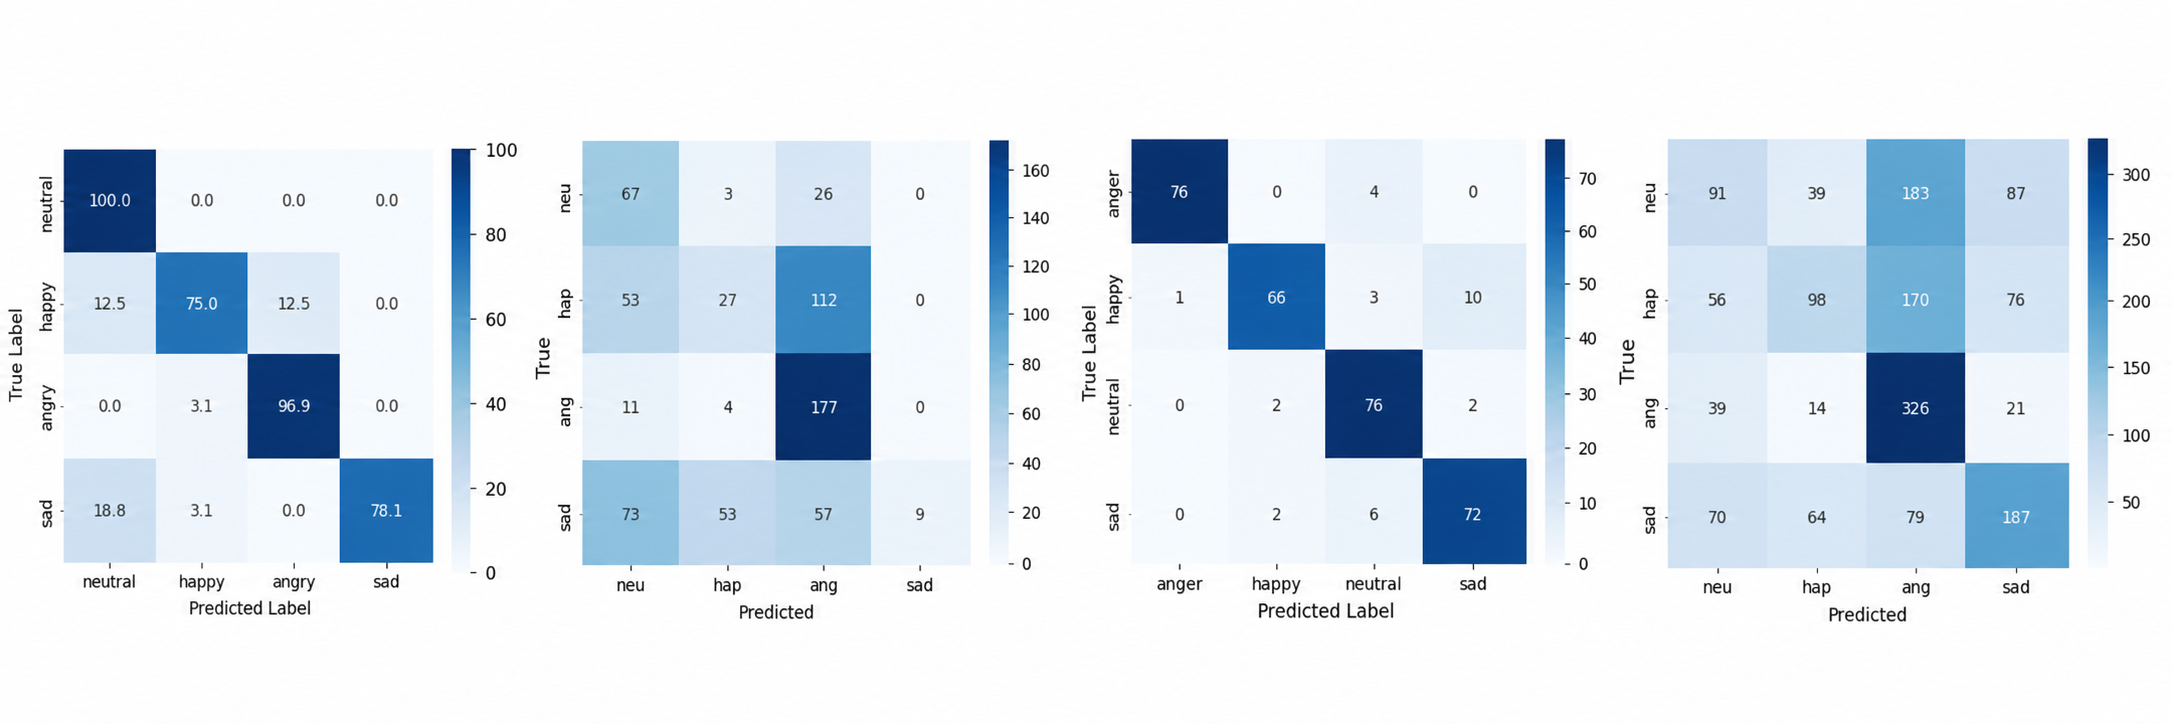
\includegraphics[width=\textwidth]{cnfall.png}
    \caption{Confusion matrices for cross-lingual speech emotion recognition: (a) English zero-shot, (b) English fine-tuned, (c) Hindi zero-shot, and (d) Hindi fine-tuned.}
    \label{fig:confusion_matrices}
\end{figure}

\subsection{Cross Lingual with Hindi Fine Tuning}

In this experiment, the model was first trained on source language and subsequently fine tuned on target language using labelled Hindi data from IESC dataset, after which testing was performed on Hindi speech. This experiment illustrates the effectiveness of target language fine tuning for domain alignment, following the procedure outlined in Algorithm~\ref{alg:finetuning}. The model achieved an accuracy of 90.62\% (Table~\ref{tab:cr_D}), indicating that fine tuning substantially improves performance by reducing phonetic and prosodic mismatch between source and target languages.

\begin{algorithm}[htbp]
\caption{Cross lingual SER with target language fine tuning}
\label{alg:finetuning}
\begin{algorithmic}[1]
\Require English dataset $D^E$, Hindi dataset $D^H$, pretrained model $f(\cdot)$
\Ensure Improved cross lingual accuracy $Acc^H$
\State Preprocess all audio signals
\State Extract features using Wav2Vec2 processor
\State Train model on source dataset $D^E$
\State Fine tune model using labeled Hindi dataset $D^H$
\State Update Transformer layers and classification head
\State Evaluate on Hindi test set $D^H_{\mathrm{test}}$
\State Compute accuracy $Acc^H$
\end{algorithmic}
\end{algorithm}

\begin{table}[htbp]
\centering
\caption{Classification report: cross lingual with Hindi fine tuning}
\label{tab:cr_D}
\renewcommand{\arraystretch}{1.2}
\begin{tabular}{lcccc}
\toprule
\textbf{Class} & \textbf{Precision} & \textbf{Recall} & \textbf{F1 score} & \textbf{Support} \\
\midrule
anger         & 0.9870 & 0.9500 & 0.9682 & 80  \\
happy         & 0.9429 & 0.8250 & 0.8880 & 80  \\
neutral       & 0.8539 & 0.9500 & 0.8994 & 80  \\
sad           & 0.8571 & 0.9000 & 0.8780 & 80  \\
\midrule
macro avg     & 0.9102 & 0.9062 & 0.9064 & 320 \\
weighted avg  & 0.9102 & 0.9062 & 0.9064 & 320 \\
\midrule
\textbf{Accuracy} & & & \textbf{0.9062} & \textbf{320} \\
\bottomrule
\end{tabular}
\end{table}

\subsection{Multilingual Analysis}

In the multilingual analysis, the pretrained Wav2Vec2 model was trained jointly on the RAVDESS (English) and IESC (Hindi) datasets, following the training procedure in Algorithm~\ref{alg:multilingual}, and subsequently evaluated on each dataset separately, with the test data held out during training to ensure evaluation on unseen samples. Testing on the IESC dataset achieved an accuracy of 90.62\%, while testing on RAVDESs achieved an accuracy of 99.5\% (Tables~\ref{tab:cr_E_IESC} and \ref{tab:cr_E_RAVDESS}, Fig.~\ref{fig:cm_E_multilingual}). These results indicate that multilingual training enhances model's ability to capture emotional characteristics compared with single language training, allowing the model to learn multilingual emotional speech patterns while preserving the pretrained acoustic representations.

\begin{algorithm}[htbp]
\caption{Multilingual training for speech emotion recognition}
\label{alg:multilingual}
\begin{algorithmic}[1]
\Require English dataset $D^E$, Hindi dataset $D^H$, pretrained model $f(\cdot)$
\Ensure Multilingual accuracies $Acc^E$, $Acc^H$
\State Preprocess audio signals from $D^E$ and $D^H$
\State Combine datasets: $D^M = D^E \cup D^H$
\State Extract features using Wav2Vec2 processor
\State Fine tune pretrained model $f(\cdot)$ on $D^M$
\State Train classification head for emotion labels
\State Evaluate on English test set $D^E_{\mathrm{test}}$ to obtain $Acc^E$
\State Evaluate on Hindi test set $D^H_{\mathrm{test}}$ to obtain $Acc^H$
\end{algorithmic}
\end{algorithm}

\begin{table}[htbp]
\centering
\caption{Classification report: multilingual analysis (IESC test)}
\label{tab:cr_E_IESC}
\renewcommand{\arraystretch}{1.2}
\begin{tabular}{lcccc}
\toprule
\textbf{Class} & \textbf{Precision} & \textbf{Recall} & \textbf{F1 score} & \textbf{Support} \\
\midrule
anger         & 0.9398 & 0.9750 & 0.9571 & 80  \\
happy         & 0.9853 & 0.8375 & 0.9054 & 80  \\
neutral       & 0.8276 & 0.9000 & 0.8623 & 80  \\
sad           & 0.8902 & 0.9125 & 0.9012 & 80  \\
\midrule
macro avg     & 0.9107 & 0.9062 & 0.9065 & 320 \\
weighted avg  & 0.9107 & 0.9062 & 0.9065 & 320 \\
\midrule
\textbf{Accuracy} & & & \textbf{0.9062} & \textbf{320} \\
\bottomrule
\end{tabular}
\end{table}

\begin{figure}[H]
    \centering
    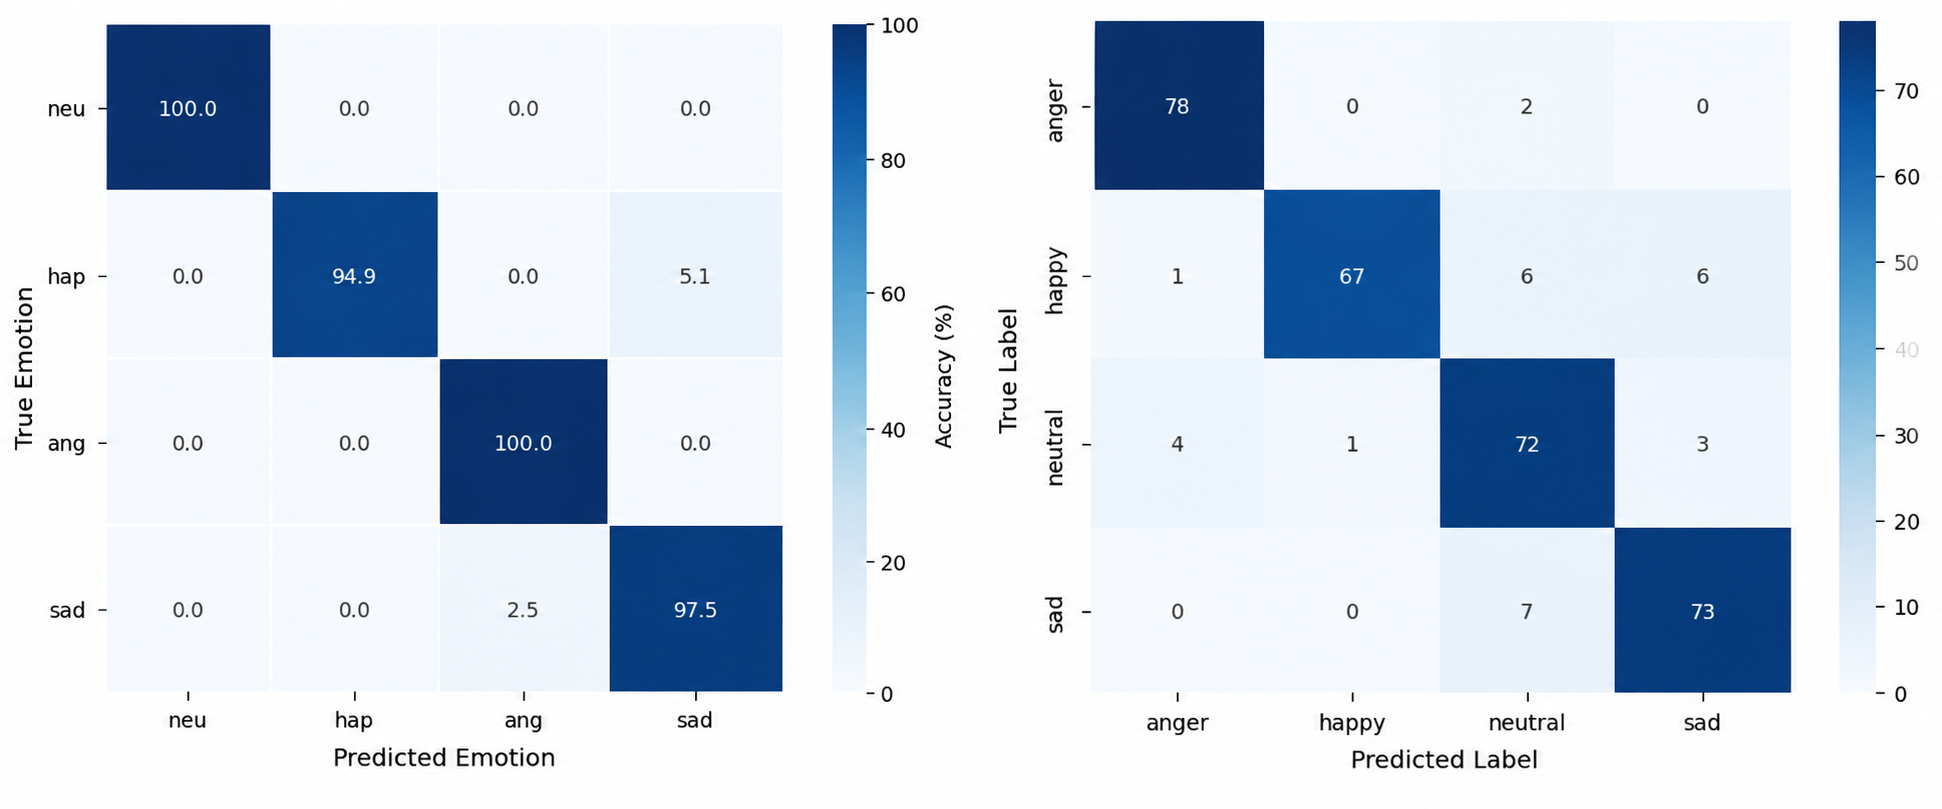
\includegraphics[width=\textwidth]{cnfm.png}
    \caption{Confusion matrices for multilingual analysis: (a) IESC test and (b) RAVDESS test.}
    \label{fig:cm_E_multilingual}
\end{figure}

\begin{table}[htbp]
\centering
\caption{Classification report: multilingual analysis (RAVDESS test)}
\label{tab:cr_E_RAVDESS}
\renewcommand{\arraystretch}{1.2}
\begin{tabular}{lcccc}
\toprule
\textbf{Class} & \textbf{Precision} & \textbf{Recall} & \textbf{F1 score} & \textbf{Support} \\
\midrule
anger         & 1.0000 & 1.0000 & 1.0000 & 192 \\
happy         & 0.9896 & 0.9948 & 0.9922 & 192 \\
neutral       & 1.0000 & 1.0000 & 1.0000 & 96  \\
sad           & 0.9948 & 0.9896 & 0.9922 & 192 \\
\midrule
macro avg     & 0.9961 & 0.9961 & 0.9961 & 672 \\
weighted avg  & 0.9955 & 0.9955 & 0.9955 & 672 \\
\midrule
\textbf{Accuracy} & & & \textbf{0.9955} & \textbf{672} \\
\bottomrule
\end{tabular}
\end{table}


\section{Discussion}
\label{sec:discussion}

The experimental results highlight effectiveness of transfer learning and fine tuning for both cross lingual and multilingual SER. When the model was evaluated directly without adaptation, performance dropped considerably, with the direct cross lingual experiments achieving accuracies of 42\% (English) and 44\% (Hindi). This indicates that model trained on one language struggles to generalize effectively to another due to substantial linguistic and acoustic differences, and demonstrates the difficulty of cross lingual emotion recognition in the absence of target language adaptation.

In contrast, fine tuning led to considerably improved accuracies. Fine tuning the pretrained model with Hindi speech data from IESC achieved accuracy of 90.6\%, representing substantial improvement over direct cross lingual setting. Similarly, fine tuning with English data from RAVDESS resulted in an accuracy of 85\%, further demonstrating the importance of target language adaptation for cross lingual emotion recognition.

The Wav2Vec2 model was found to be well suited to multilingual analysis, outperforming the cross lingual configurations, with accuracies of 90.62\% on IESC and 99.5\% on RAVDESS. This suggests that a model trained jointly across languages is better able to recognize emotions irrespective of the language of the input speech. Such systems could be beneficial for call centre analytics, emotion aware human-computer interaction, and mental health support tools, particularly in settings where linguistic resources are limited.


\section{Conclusion}
\label{sec:conclusion}

This paper examined the limitations of current SER systems using English (RAVDESS) and Hindi (IESC) speech data. Multilingual and cross lingual evaluation using the pretrained Wav2Vec 2.0 model showed that direct cross lingual transfer without fine tuning yields low accuracy, owing to linguistic and acoustic variation between the two languages. Fine tuning on a small fraction target language considerably improved performance for both English and Hindi, and multilingual training, in which the model was trained jointly on both languages, achieved the strongest overall results. These findings are expected to be useful for the design of robust SER systems for languages with limited or no labelled data.

Future work will explore attention based transformer architectures, incorporate larger multilingual speech corpora, and employ parameter-efficient fine-tuning approaches such as LoRA to reduce training cost. Extending this study to additional Indian languages such as Tamil and Bengali would further broaden the applicability of SER for Indian speakers.

\begin{credits}
\subsubsection{\discintname}
Authors have no competing interests to declare that are relevant to the content of this article.
\end{credits}


\begin{thebibliography}{19}

\bibitem{b1}
Zaidi, M., Latif, S., Qadir, J.: Cross-language speech emotion recognition using multimodal dual attention transformers. arXiv preprint arXiv:2306.13804 (2023)

\bibitem{b2}
Ryumina, E., Axyonov, A., Abdulkadirov, T., Koryakovskaya, D., Ryumin, D.: Cross-lingual bimodal emotion recognition with LLM-based label smoothing. Big Data Cogn. Comput. \textbf{9}(11), 285 (2025). \doi{10.3390/bdcc9110285}

\bibitem{b3}
Upadhyay, S.G., Martinez-Lucas, L., Katz, W., Busso, C., Lee, C.-C.: Phonetically-anchored domain adaptation for cross-lingual speech emotion recognition. IEEE Trans. Affect. Comput. \textbf{16}(3), 1631--1645 (2025)

\bibitem{b4}
Agarla, M., Bianco, S., Celona, L., Napoletano, P., Petrovsky, A., Piccoli, F., Schettini, R., Shanin, I.: Semi-supervised cross-lingual speech emotion recognition. Expert Syst. Appl. \textbf{237}, 121368 (2024)

\bibitem{b7}
Latif, S., Rana, R., Khalifa, S., Jurdak, R., Schuller, B.W.: Self supervised adversarial domain adaptation for cross-corpus and cross-language speech emotion recognition. IEEE Trans. Affect. Comput. \textbf{14}(3), 1912--1926 (2023)

\bibitem{b8}
Latif, S., Qadir, J., Bilal, M.: Unsupervised adversarial domain adaptation for cross-lingual speech emotion recognition. In: 2019 8th International Conference on Affective Computing and Intelligent Interaction (ACII), pp. 732--737. IEEE, Cambridge, UK (2019)

\bibitem{b9}
Liu, J., Zheng, W., Zong, Y., Lu, C., Tang, C.: Cross corpus speech emotion recognition based on deep domain adaptive convolutional neural network. IEICE Trans. Inf. Syst. \textbf{103-D}(2), 459--463 (2020)

\bibitem{b11}
D'Asaro, F., M\'{a}rquez Villac\'{i}s, J.J., Rizzo, G., Bottino, A.: Using large speech models for feature extraction in cross-lingual speech emotion recognition. In: Proceedings of the 10th Italian Conference on Computational Linguistics (CLiC-it 2024), pp. 258--265. CEUR Workshop Proceedings, Pisa, Italy (2024)

\bibitem{b12}
Ahn, Y., Lee, S.J., Shin, J.W.: Cross-corpus speech emotion recognition based on few-shot learning and domain adaptation. IEEE Signal Process. Lett. \textbf{28}, 1190--1194 (2021)

\bibitem{b13}
Zhao, H., Ye, N., Wang, R.: Improved cross-corpus speech emotion recognition using deep local domain adaptation. Chinese J. Electron. \textbf{32}(3), 640--646 (2023)

\bibitem{b14}
Cai, X., Wu, Z., Zhong, K., Su, B., Dai, D., Meng, H.: Unsupervised cross-lingual speech emotion recognition using domain adversarial neural network. In: 2021 12th International Symposium on Chinese Spoken Language Processing (ISCSLP), pp. 1--5. IEEE, Hong Kong (2021)

\bibitem{b15}
Abdelwahab, M., Busso, C.: Domain adversarial for acoustic emotion recognition. IEEE/ACM Trans. Audio Speech Lang. Process. \textbf{26}(12), 2423--2435 (2018)

\bibitem{b16}
Babu, A., Wang, C., Tjandra, A., et al.: XLS-R: self-supervised cross-lingual speech representation learning at scale. arXiv preprint arXiv:2111.09296 (2021)

\bibitem{b17}
Sharma, M.: Multi-lingual multi-task speech emotion recognition using Wav2Vec 2.0. In: 2022 IEEE International Conference on Acoustics, Speech and Signal Processing (ICASSP), pp. 6907--6911. IEEE, Singapore (2022)

\bibitem{b18}
Bhattacharya, S., Borah, S., Mishra, B.K., Das, N.: Deep analysis for speech emotion recognization. In: 2022 Second International Conference on Computer Science, Engineering and Applications (ICCSEA), pp. 1--6. IEEE, Gunupur, India (2022)

\bibitem{b22}
Bhattacharya, S., Mishra, B.K., Borah, S., Das, N., Dey, N.: Cross-lingual deep learning model for gender-based emotion detection. Multimedia Tools and Applications \textbf{83}(9), 25969--26007 (2024)

\bibitem{b23}
Jafarzadeh, P., Rostami, A.M., Choobdar, P.: Speaker emotion recognition: leveraging self-supervised models for feature extraction using Wav2Vec2 and HuBERT. arXiv preprint arXiv:2411.02964 (2024)

\bibitem{b27}
Chen, S., Wang, C., Chen, Z., et al.: WavLM: large-scale self-supervised pre-training for full stack speech processing. IEEE J. Sel. Top. Signal Process. \textbf{16}(6), 1505--1518 (2022)

\bibitem{b28}
Shendabadi, A., Izadirad, P., Salehi, M., Bijankhan, M.: Speech emotion recognition leveraging OpenAI's Whisper representations and attentive pooling methods. arXiv preprint arXiv:2602.06000 (2026)

\end{thebibliography}

\end{document}